\part{Results}
\section{Results}

\begin{frame}
	\partpage
	\centering
\end{frame}

%%%%%%%%%%%%%%%%%%%%%%%%%%%%%%%%%%%%%%%%%%%%%%%%%%%%%%%%%%%%%%%%%%%%%%%%%%%%%%%%%%%%%%%%%%%%%%%%%%%%%%%%%%%%%%%%%%%%%%%%%%%
%%%%%%%%%%%%%%%%%%%%%%%%%%%%%%%%%%%%%%%%%%%%%%%%%%%%%%%%%%%%%%%%%%%%%%%%%%%%%%%%%%%%%%%%%%%%%%%%%%%%%%%%%%%%%%%%%%%%%%%%%%%

\begin{frame}
	\frametitle{Source code \& Dataset}
	\centering
	
	Original source code by medvedev group available on:\\
	
	\medskip
	
	{\color{blue}https://github.com/medvedevgroup/TwoPaCo} \\
	
	\medskip
  \noindent\rule{4cm}{0.4pt}
	\medskip
	
	Personal implementation and presentation available on:\\
	\medskip

	{\color{blue}https://github.com/GaspareG/TwoPaCo}

	\medskip
	
	{\color{blue}https://github.com/GaspareG/TwoPaCoPresentation}
	
	\medskip
  \noindent\rule{4cm}{0.4pt}
	\medskip
		
	Dataset for experiments:

	\medskip
	
	62 Escherichia coli ({\color{green}$\sim$300Mb})\\
	5 humans ({\color{orange}$\sim$21Gb})\\
  8 primates ({\color{orange}$\sim$23Gb})\\
  100 simulated human ({\color{red}$\sim$400Gb})
	
	
\end{frame}

%%%%%%%%%%%%%%%%%%%%%%%%%%%%%%%%%%%%%%%%%%%%%%%%%%%%%%%%%%%%%%%%%%%%%%%%%%%%%%%%%%%%%%%%%%%%%%%%%%%%%%%%%%%%%%%%%%%%%%%%%%%
%%%%%%%%%%%%%%%%%%%%%%%%%%%%%%%%%%%%%%%%%%%%%%%%%%%%%%%%%%%%%%%%%%%%%%%%%%%%%%%%%%%%%%%%%%%%%%%%%%%%%%%%%%%%%%%%%%%%%%%%%%%

\begin{frame}
  
	\frametitle{Memory complexity}

  \centering
	
	The memory complexity is the maximum \\ among the first and the second pass of TwoPaCo \\
	
	\medskip
	
	\begin{itemize}
	  \item[\textcolor{green}{\textbullet}] First pass: insert all $k$-mers in a bloom filter of \textbf{size $b$}
	  \item[\textcolor{orange}{\textbullet}] Second pass: store all \textbf{junction candidates} in a hash table
	\end{itemize}
	
	\medskip
	
	\pause
	
	How many junction candidates?
	
	\begin{itemize}
	  \item Real junction, $J$
	  \item False positive induced from the bloom filter, $FP$
	\end{itemize}

	\medskip
	
	\pause
	
	Result: $\mathcal{O}(\max\{{\color{green}b}, {\color{orange}(J+FP)k}\})$
	
	
\end{frame}

%%%%%%%%%%%%%%%%%%%%%%%%%%%%%%%%%%%%%%%%%%%%%%%%%%%%%%%%%%%%%%%%%%%%%%%%%%%%%%%%%%%%%%%%%%%%%%%%%%%%%%%%%%%%%%%%%%%%%%%%%%%
%%%%%%%%%%%%%%%%%%%%%%%%%%%%%%%%%%%%%%%%%%%%%%%%%%%%%%%%%%%%%%%%%%%%%%%%%%%%%%%%%%%%%%%%%%%%%%%%%%%%%%%%%%%%%%%%%%%%%%%%%%%

\begin{frame}
  
	\frametitle{Time complexity}

  \centering
	
	The time complexity is the sum \\ between the first and the second pass of TwoPaCo \\
	
	\bigskip
	
	\begin{itemize}
	  \item[\textcolor{green}{\textbullet}]First pass: \textbf{insert all $k$-mers} in a bloom filter using $h$ hash functions
	  \item[\textcolor{orange}{\textbullet}] Second pass: iterate over all \textbf{candidate positions} and query the hash table
	\end{itemize}
	
	\bigskip
	
	\pause
	
	How many $k$-mers? \\
	
	$\mathcal{O}(m)$, where $m = \Sigma_{s \in S}{ |s| }$ is the total input size
	
	\bigskip
	 
	\pause
	
	How many candidate positions?
	
	\begin{itemize}
	  \item Real positions, $|G_{c}|$
	  \item False positive induced from the bloom filter, $FP$
	\end{itemize}

	\medskip
	
	\pause
	
	Result: $\mathcal{O}({\color{green}mh} + {\color{orange}(|G_{c}| + FP)k})$
	
	
\end{frame}


%%%%%%%%%%%%%%%%%%%%%%%%%%%%%%%%%%%%%%%%%%%%%%%%%%%%%%%%%%%%%%%%%%%%%%%%%%%%%%%%%%%%%%%%%%%%%%%%%%%%%%%%%%%%%%%%%%%%%%%%%%%
%%%%%%%%%%%%%%%%%%%%%%%%%%%%%%%%%%%%%%%%%%%%%%%%%%%%%%%%%%%%%%%%%%%%%%%%%%%%%%%%%%%%%%%%%%%%%%%%%%%%%%%%%%%%%%%%%%%%%%%%%%%

\begin{frame}
	\frametitle{Complexity comparison}
	
	\centering
	
	%\pause
	
  State of the art for compressed de Bruijn graph construction:
  
	  \begin{itemize}
	    \item Sibelia (Minkin, Patel, Kolmogorov, Vyahhi, Pham, 2013)
	    \item SplitMEM (Marcus, Lee, Schatz, 2014)
	    \item bwt-based (Baier, Beller, Ohlebusch, 2015)
	  \end{itemize}

	  \pause	
	
	  \medskip
	  
    \scalebox{0.85}{                        
  
  	  \begin{tabular}{ | r | r | r | }
    \hline
    Algorithm  &                      Time complexity &        Memory complexity   \\ \hline
    Sibelia    & $\mathcal{O}(m)$                    & $\mathcal{O}({\color{red}m})$                     \\
    SplitMEM   & $\mathcal{O}(m \log{g})$            & $\mathcal{O}(|G_{c}|+{\color{red}m})$           \\
    bwt-based  & $\mathcal{O}(m)$                    & $\mathcal{O}({\color{red}m})$                     \\
    TwoPaCo    & $\mathcal{O}(mh + (|G_{c}| + FP)k)$ & $\mathcal{O}(\max\{b, (J+FP)k \})$ \\    
    \hline
    \end{tabular}
  
    }
        
    \medskip

	%\pause
	
    \begin{itemize}
      \item $m = \Sigma_{s \in S}{ |s| }$, total input size
      \item $g = \max_{s \in S}{ |s| }$, size of the biggest genoma
      \item $J$ and $|G_{c}|$, number of vertex and edge in the de Bruijn Graph
      \item $b$ and $h$, size of the bloom filter table and number of hash functions
      \item $FP$, number of false positives in first pass
    \end{itemize}
    

\end{frame}

%%%%%%%%%%%%%%%%%%%%%%%%%%%%%%%%%%%%%%%%%%%%%%%%%%%%%%%%%%%%%%%%%%%%%%%%%%%%%%%%%%%%%%%%%%%%%%%%%%%%%%%%%%%%%%%%%%%%%%%%%%%
%%%%%%%%%%%%%%%%%%%%%%%%%%%%%%%%%%%%%%%%%%%%%%%%%%%%%%%%%%%%%%%%%%%%%%%%%%%%%%%%%%%%%%%%%%%%%%%%%%%%%%%%%%%%%%%%%%%%%%%%%%%
\begin{frame}
	\frametitle{Running time comparison}

	\centering

  What are the practical performances of TwoPaCo against the state of the art? \\

  \pause
  
  \medskip  	

	  \scalebox{.7}{                        

    \begin{tabular}{ | r | r | r | r | r | r | r | }
    \hline
    Dataset    &  Sibelia &   SplitMEM &     bwt-based &  \multicolumn{2}{c|}{TwoPaCo} \\ \hline
    \multicolumn{4}{| r |}{}                           & 1 thread & 15 thread\\ \hline
               
    62 E.coli (k=25)   & 10 ({\color{orange}12.2}) & 70 ({\color{red}178.0}) &      8 ({\color{orange}0.85}) &    4 ({\color{green}0.16}) & 2 (0.39) \\
    62 E.coli (k=100)  &   8 ({\color{orange}7.6}) & 67 ({\color{red}178.0}) &      8 ({\color{orange}0.50}) &    4 ({\color{green}0.19}) & 2 (0.39) \\ \hline
    
    7 humans (k=25)    &        - &          - &  867 ({\color{red}100.30}) &  436 ({\color{green}4.40}) & 63 (4.84) \\ 
    7 humans (k=100)   &        - &          - &   807 ({\color{red}46.02}) &  317 ({\color{green}8.42}) & 57 (8.75) \\ \hline
    
    8 primates (k=25)  &        - &          - &             - & 914 ({\color{green}34.36}) & 111 (34.36) \\
    8 primates (k=100) &        - &          - &             - & 756 ({\color{green}56.06}) & 101 (61.68) \\ \hline
    
    50 humans (k=25)   &        - &          - &             - &          -  & 705 (69.77) \\
    50 humans (k=100)  &        - &          - &             - &          -  & 927 (70.21) \\ \hline
     
    \end{tabular}
    
    }

    \medskip

    Running times in minutes and memory usage in gigabytes in parenthesis
        
    \medskip
    
    \begin{itemize}
      \item - on Sibelia = out of time
      \item - on SplitMEM = out of memory
      \item - on bwt-based = out of memory
      \item - on TwoPaCo = experiment not done
    \end{itemize}

\end{frame}

%%%%%%%%%%%%%%%%%%%%%%%%%%%%%%%%%%%%%%%%%%%%%%%%%%%%%%%%%%%%%%%%%%%%%%%%%%%%%%%%%%%%%%%%%%%%%%%%%%%%%%%%%%%%%%%%%%%%%%%%%%%
%%%%%%%%%%%%%%%%%%%%%%%%%%%%%%%%%%%%%%%%%%%%%%%%%%%%%%%%%%%%%%%%%%%%%%%%%%%%%%%%%%%%%%%%%%%%%%%%%%%%%%%%%%%%%%%%%%%%%%%%%%%

\begin{frame}
	\frametitle{Fixed memory}
	\centering
	
	In how many rounds do we need to split the input\\ to not exceeding a given memory threshold?
	
	\pause

	\bigskip
		
	\begin{tabular}{ | r | r | r | r | r | }
  \hline
  Threshold  & Used memory & Bloom filter size & Running time & Rounds \\ \hline
  {\color{red}10GB}   &      8.62GB &       8.59GB ($2^{33}$) & {\color{green}4h} &      1 \\
  {\color{orange}8GB} &      6.73GB &       4.29GB ($2^{32}$) & {\color{orange}7h} &      3 \\
  {\color{orange}6GB} &      5.98GB &       4.29GB ($2^{32}$) & {\color{orange}9h} &      4 \\
  {\color{green}4GB}  &      3.51GB &       2.14GB ($2^{31}$) & {\color{red}11h} &      6 \\
  \hline
  \end{tabular}
  
  \medskip
  
  Experiments on 5 simulated human genomes, $k = 25$, 8 threads
  
  \medskip
  
  \pause
  
  Result: \textbf{we can trade-off memory for time}
  

\end{frame}

%%%%%%%%%%%%%%%%%%%%%%%%%%%%%%%%%%%%%%%%%%%%%%%%%%%%%%%%%%%%%%%%%%%%%%%%%%%%%%%%%%%%%%%%%%%%%%%%%%%%%%%%%%%%%%%%%%%%%%%%%%%
%%%%%%%%%%%%%%%%%%%%%%%%%%%%%%%%%%%%%%%%%%%%%%%%%%%%%%%%%%%%%%%%%%%%%%%%%%%%%%%%%%%%%%%%%%%%%%%%%%%%%%%%%%%%%%%%%%%%%%%%%%%

%\begin{frame}
%	\frametitle{Parallel scalability}
%	\centering
%	
%	How does the performance of TwoPaCo improve \\to the increasing of working threads?
%	 
%	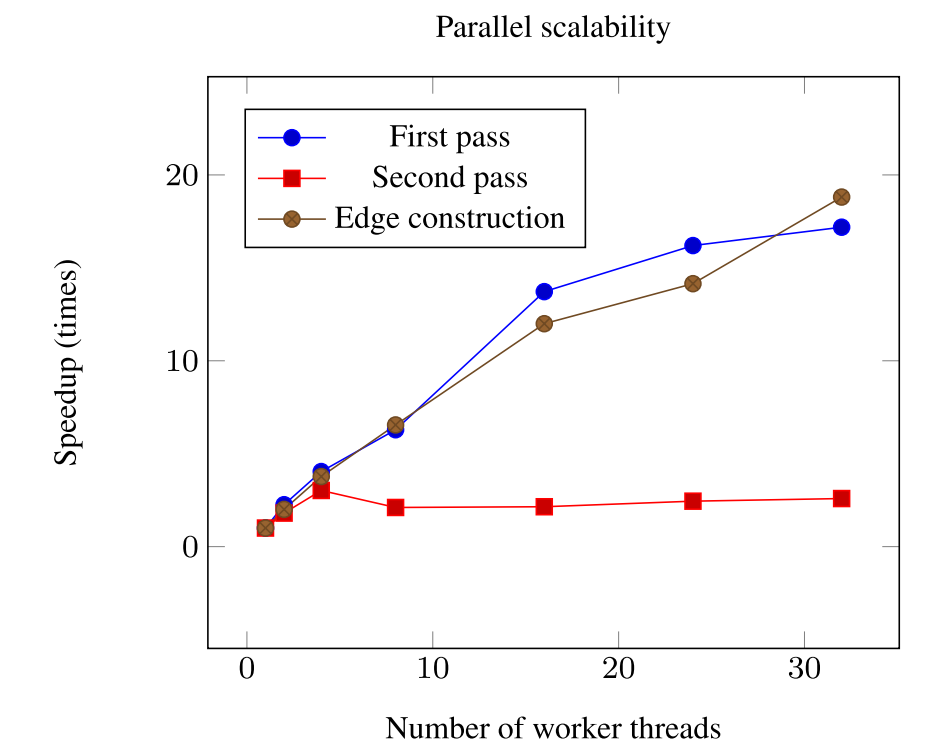
\includegraphics[height=5cm]{images/scalability}
%	
%	\begin{itemize}
%	  \item First pass: great improvement thanks to concurrent bloom filter
%	  \item Second pass: slight improvement due to race-conditions on the hash table
%	  \item Edge construction: great improvement thanks to $k$-mers independency
%	\end{itemize}
%\end{frame}

%%%%%%%%%%%%%%%%%%%%%%%%%%%%%%%%%%%%%%%%%%%%%%%%%%%%%%%%%%%%%%%%%%%%%%%%%%%%%%%%%%%%%%%%%%%%%%%%%%%%%%%%%%%%%%%%%%%%%%%%%%%
%%%%%%%%%%%%%%%%%%%%%%%%%%%%%%%%%%%%%%%%%%%%%%%%%%%%%%%%%%%%%%%%%%%%%%%%%%%%%%%%%%%%%%%%%%%%%%%%%%%%%%%%%%%%%%%%%%%%%%%%%%%

\begin{frame}
	\frametitle{Bloom Filter false positive}
	\centering
	
	  Is the Bloom Filter really efficient in reducing junction candidates?
	  
	  \pause
	  
    \bigskip
	  
	  %\scalebox{.7}{                        
    %\begin{tabular}{ r | r | r | r | r | r }
    %\hline
    %Dataset    &   k &            Initial &       First pass &      Second pass & \%Fp \\ \hline
    %62 E.coli  &  25 &  $3.101 * 10^{8\phantom{0}}$  & $2.464 * 10^{7}$ & $2.457 * 10^{7}$ & \phantom{0}0.31\% \\
    %62 E.coli  & 100 &  $3.101 * 10^{8\phantom{0}}$  & $2.284 * 10^{7}$ & $9.492 * 10^{6}$ & 58.45\% \\
    %7 humans   &  25 &  $2.120 * 10^{10}$ & $3.489 * 10^{9}$ & $2.974 * 10^{9}$ & 14.78\% \\
    %7 humans   & 100 &  $2.120 * 10^{10}$ & $1.374 * 10^{9}$ & $1.882 * 10^{8}$ & 86.30\% \\
    %8 primates &  25 &  $2.454 * 10^{10}$ & $5.423 * 10^{9}$ & $5.401 * 10^{9}$ & \phantom{0}0.39\% \\
    %8 primates & 100 &  $2.454 * 10^{10}$ & $1.174 * 10^{9}$ & $5.024 * 10^{8}$ & 57.20\% \\ \hline
    %\end{tabular}
    %}
    
    %\scalebox{.7}{                        
    %\begin{tabular}{ r | r | r | r | r | r }
    %\hline
    %           &     &    \multicolumn{3}{ c | }{Junction candidates} &                \\ \hline
    %Dataset    &   k &        Initial &    First pass &   Second pass & False positive \\ \hline
    %62 E.coli  &  25 &    310 157 564 &    24 649 489 &    24 572 562 &         76 927 \\ 
    %62 E.coli  & 100 &    310 157 489 &    22 848 018 &     9 492 091 &     13 355 927 \\ \hline
    %7 humans   &  25 & 21 201 290 922 & 3 489 946 013 & 2 974 098 154 &    515 847 859 \\ 
    %7 humans   & 100 & 21 201 290 847 & 1 374 287 870 &   188 224 214 &  1 186 063 656 \\ \hline
    %8 primates &  25 & 24 540 556 921 & 5 423 003 377 & 5 401 587 503 &     21 415 874 \\ 
    %8 primates & 100 & 24 540 556 846 & 1 174 160 336 &   502 441 107 &    671 719 229 \\ \hline
    %        
    %\end{tabular}
    %}
    
    \scalebox{.7}{                        
    \begin{tabular}{ r | r | r | r | r }
    \hline
               &     &                                  \multicolumn{3}{ c }{Junction candidates} \\ \hline
    Dataset    &   k &                Initial &              First pass &             Second pass \\ \hline
    62 E.coli  &  25 &    310 157 564 ({\color{red}100\%}) &    24 649 489  ({\color{orange}7.94\%}) &    24 572 562  ({\color{green}7.92\%}) \\ 
    62 E.coli  & 100 &    310 157 489 (100\%) &    22 848 018  (7.36\%) &     9 492 091  (3.06\%) \\ \hline
    7 humans   &  25 & 21 201 290 922 ({\color{red}100\%}) & 3 489 946 013 ({\color{orange}16.46\%}) & 2 974 098 154 ({\color{green}14.02\%}) \\ 
    7 humans   & 100 & 21 201 290 847 (100\%) & 1 374 287 870  (6.48\%) &   188 224 214  (0.88\%) \\ \hline
    8 primates &  25 & 24 540 556 921 ({\color{red}100\%}) & 5 423 003 377 ({\color{orange}22.09\%}) & 5 401 587 503 ({\color{green}22.01\%}) \\ 
    8 primates & 100 & 24 540 556 846 (100\%) & 1 174 160 336  (4.78\%) &   502 441 107  (2.04\%) \\ \hline
            
    \end{tabular}
    }
    
    %\caption{Reduction of junction candidates}
    
    \bigskip
    
    \begin{itemize}
      \item Initial: total number of $k$-mers in dataset
      \item First pass: number of junction candidates (using a bloom filter)
      \item Second pass: real number of junction (using an hash table)
      %\item False positive: (Second pass - First pass)
    \end{itemize}
        
\end{frame}

%%%%%%%%%%%%%%%%%%%%%%%%%%%%%%%%%%%%%%%%%%%%%%%%%%%%%%%%%%%%%%%%%%%%%%%%%%%%%%%%%%%%%%%%%%%%%%%%%%%%%%%%%%%%%%%%%%%%%%%%%%%
%%%%%%%%%%%%%%%%%%%%%%%%%%%%%%%%%%%%%%%%%%%%%%%%%%%%%%%%%%%%%%%%%%%%%%%%%%%%%%%%%%%%%%%%%%%%%%%%%%%%%%%%%%%%%%%%%%%%%%%%%%%

\begin{frame}
	\frametitle{Conclusion}
	\centering

  \begin{itemize}
    \item Lowest time/memory usage in the state of the art
    \item Highly scalable (best performance with multi-thread CPUs)
    \item Time/memory trade-off (suitable for small computer)
    \item Bloom filter perform very well in practice
  \end{itemize}

\end{frame}
